%!TEX program = xelatex

\documentclass[11pt,titlepage]{report}
%!TEX root = main.tex

\usepackage[T1]{fontenc}
\usepackage{lmodern}
\usepackage[svgnames]{xcolor}
\usepackage{fontspec} % XeLaTeX required!
\usepackage{graphicx}
\usepackage{circuitikz}
\usepackage{tikz}
\usepackage{pifont}
\usepackage[some]{background}
\usepackage{xltxtra} 
\usepackage{setspace}
\usepackage[absolute]{textpos}
\usepackage[latin1]{inputenc}
\usepackage[english]{babel}
\usepackage{graphicx}
\usepackage{wrapfig}
\usepackage{fullpage}
\usepackage[margin=1in]{geometry}
\usepackage{float}
\usepackage{url}
\usepackage{multicol}
\usepackage{hyperref}
\usepackage{titlepic}
\usepackage{standalone}
\usepackage{siunitx}
\usepackage{booktabs}
\usepackage{amsmath}
\usepackage{unicode-math}
\usepackage{verbatim}
\usepackage{enumitem}
\usepackage{listings}
\usepackage{multirow}
\usepackage{pgfplots}
\pgfplotsset{compat=1.8}
\usepackage{caption} 
\usepackage[parfill]{parskip}
\usepackage{import}
\usepackage[backend=bibtexu,texencoding=utf8,bibencoding=utf8,style=ieee,sortlocale=en_GB,language=auto]{biblatex}
\usepackage[strict,autostyle]{csquotes}
\usepackage[final]{pdfpages}
\usepackage{subcaption}
\usepackage{ifplatform}
%\captionsetup[table]{skip=10pt}


% Fix for includepdf bug in Mac OS X
\newcommand{\insertpdfpath}[1]{
	\ifwindows
	\newcommand{\insertpdf}[2]{\includepdf[pages=##1]{##2}}
	\else
	\newcommand{\insertpdf}[2]{\includepdf[pages=##1]{#1/##2}}
	\fi
}

%set fonts
\setmainfont[Ligatures=TeX]{Myriad Pro}
\setmathfont{Asana Math}
\setmonofont{Lucida Console}

\usepackage{titlesec, color}
\renewcommand{\familydefault}{\sfdefault} %set font family
\renewcommand{\arraystretch}{1.2} %set table vertical spacing
\setlength\parindent{0pt} %no paragraph indent
\hypersetup{ %setup hyperlinks
    colorlinks,
    citecolor=black,
    filecolor=black,
    linkcolor=black,
    urlcolor=black
}

%redesign chapter headings
\definecolor{gray75}{gray}{0.75}
\newcommand{\chapternumber}{\thechapter}
\newcommand{\hsp}{\hspace{20pt}}
\titleformat{\chapter}[hang]{\Huge\bfseries}{\chapternumber\hsp\textcolor{gray75}{|}\hsp}{0pt}{\Huge\bfseries}

%Redefine appendix headers
\renewcommand{\appendixname}{Appendix}
\renewcommand{\appendixtocname}{Appendices}
\renewcommand{\appendixpagename}{Appendices}

%For code listings
\definecolor{black}{rgb}{0,0,0}
\definecolor{browntags}{rgb}{0.65,0.1,0.1}
\definecolor{bluestrings}{rgb}{0,0,1}
\definecolor{graycomments}{rgb}{0.4,0.4,0.4}
\definecolor{redkeywords}{rgb}{1,0,0}
\definecolor{bluekeywords}{rgb}{0.13,0.13,0.8}
\definecolor{greencomments}{rgb}{0,0.5,0}
\definecolor{redstrings}{rgb}{0.9,0,0}
\definecolor{purpleidentifiers}{rgb}{0.01,0,0.01}


\lstdefinestyle{csharp}{
language=[Sharp]C,
showspaces=false,
showtabs=false,
breaklines=true,
showstringspaces=false,
breakatwhitespace=true,
escapeinside={(*@}{@*)},
columns=fullflexible,
commentstyle=\color{greencomments},
keywordstyle=\color{bluekeywords}\bfseries,
stringstyle=\color{redstrings},
identifierstyle=\color{purpleidentifiers},
basicstyle=\ttfamily\small}

\lstdefinestyle{c}{
language=C,
showspaces=false,
showtabs=false,
breaklines=true,
showstringspaces=false,
breakatwhitespace=true,
escapeinside={(*@}{@*)},
columns=fullflexible,
commentstyle=\color{greencomments},
keywordstyle=\color{bluekeywords}\bfseries,
stringstyle=\color{redstrings},
identifierstyle=\color{purpleidentifiers},
}

\lstdefinestyle{matlab}{
language=Matlab,
showspaces=false,
showtabs=false,
breaklines=true,
showstringspaces=false,
breakatwhitespace=true,
escapeinside={(*@}{@*)},
columns=fullflexible,
commentstyle=\color{greencomments},
keywordstyle=\color{bluekeywords}\bfseries,
stringstyle=\color{redstrings},
identifierstyle=\color{purpleidentifiers}
}

\lstdefinestyle{vhdl}{
language=VHDL,
showspaces=false,
showtabs=false,
breaklines=true,
showstringspaces=false,
breakatwhitespace=true,
escapeinside={(*@}{@*)},
columns=fullflexible,
commentstyle=\color{greencomments},
keywordstyle=\color{bluekeywords}\bfseries,
stringstyle=\color{redstrings},
identifierstyle=\color{purpleidentifiers}
}

\lstdefinestyle{xaml}{
language=XML,
showspaces=false,
showtabs=false,
breaklines=true,
showstringspaces=false,
breakatwhitespace=true,
escapeinside={(*@}{@*)},
columns=fullflexible,
commentstyle=\color{greencomments},
keywordstyle=\color{redkeywords},
stringstyle=\color{bluestrings},
tagstyle=\color{browntags},
morestring=[b]",
  morecomment=[s]{<?}{?>},
  morekeywords={xmlns,version,typex:AsyncRecords,x:Arguments,x:Boolean,x:Byte,x:Char,x:Class,x:ClassAttributes,x:ClassModifier,x:Code,x:ConnectionId,x:Decimal,x:Double,x:FactoryMethod,x:FieldModifier,x:Int16,x:Int32,x:Int64,x:Key,x:Members,x:Name,x:Object,x:Property,x:Shared,x:Single,x:String,x:Subclass,x:SynchronousMode,x:TimeSpan,x:TypeArguments,x:Uid,x:Uri,x:XData,Grid.Column,Grid.ColumnSpan,Click,ClipToBounds,Content,DropDownOpened,FontSize,Foreground,Header,Height,HorizontalAlignment,HorizontalContentAlignment,IsCancel,IsDefault,IsEnabled,IsSelected,Margin,MinHeight,MinWidth,Padding,SnapsToDevicePixels,Target,TextWrapping,Title,VerticalAlignment,VerticalContentAlignment,Width,WindowStartupLocation,Binding,Mode,OneWay,xmlns:x}
}

\lstdefinestyle{matlab}{
language=Matlab,
showspaces=false,
showtabs=false,
breaklines=true,
showstringspaces=false,
breakatwhitespace=true,
escapeinside={(*@}{@*)},
columns=fullflexible,
commentstyle=\color{greencomments},
keywordstyle=\color{bluekeywords}\bfseries,
stringstyle=\color{purpleidentifiers},
identifierstyle=\color{purpleidentifiers}
}

%defaults
\lstset{
basicstyle=\ttfamily\small,
extendedchars=false,
numbers=left,
numberstyle=\ttfamily\tiny,
stepnumber=1,
tabsize=4,
numbersep=5pt
}
\addbibresource{../../library/bibliography.bib}

\newcommand{\figpath}{../../deliverable-7-resources/figures}

\begin{document}

\chapter{Assignment 2}
\section{Labday 4}

\subsection{Report 1}
\label{subsec:ass-2-rep-1}
Detection of the smallest phase difference possible between two sound waves occurs in the situation where the waves peak in two successive samples. This means that the time difference between their peaks, which is the time that one wave lags, or leads, the other, is at least the sample period. Therefore, the spatial resolution $\Delta \lambda$ is given by $\Delta \lambda = v T_s$, where $v \approx$ \SI{343.9}{m/s} denotes the speed of sound and $T_s$ the sample period. Consequently, for a spatial resolution of \SI{1}{cm}, a sample frequency $F_s = 1/T_s$ of \SI{34.4}{kHz} is required. With a sample frequency of \SI{44.1}{kHz}, one obtains a spatial resolution of \SI{0.78}{cm}, which seems fine. The amount of samples corresponding to a maximal propagation delay of \SI{5}{m} will then be \num{642}.

The length of a typical impulse response is approximately \SI{10}{ms}, which follows from a maximal propagation delay of roughly \SI{5}{m} and the graphs shown in Subsection \ref{subsec:ass-1-rep-13}. Therefore, we chose \texttt{timer3} to be \SI{8}{Hz} so that the repetition period easily contains the impulse response. We then chose \texttt{timer0} to be \SI{15}{kHz} in combination with \texttt{timer1} \SI{3}{kHz} so that \textbf{(1)}, the resulting spectrum will not be disturbed by human speech too much, \textbf{(2)}, the resulting spectrum will not be filtered by audio filters and \textbf{(3)}, the sent signal's length is still around \SI{10}{ms}.

\subsection{Report 2}
We implemented a localization method which makes use of deconvolution by inversion and a peak detection algorithm to determine the LOS time difference of arrivals of the received signals. Figure~\ref{fig:ass-2-rep-2-typical} shows a typical data segment.

\begin{figure}[H]
	\begin{center}
		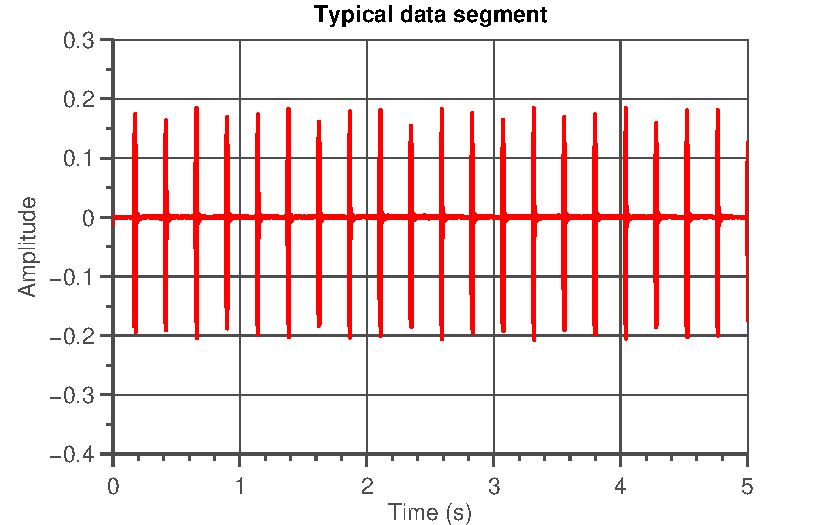
\includegraphics[width=.6\linewidth]{\figpath/ass-2/report-2-3/ass-2-report-2-typical-data-segment.pdf}
	\end{center}
	\caption{A typical data segment}
	\label{fig:ass-2-rep-2-typical}
\end{figure}

By means of the described localization method, we tried to determine the spacing between two microphones. The recovered impulse responses are shown in Figure \ref{fig:ass-2-rep-2-imps}. Note that the amplitudes are shown logarithmic to increase readability of the graphs.

\begin{figure}[H]
	\centering
	\begin{subfigure}{.49\textwidth}
		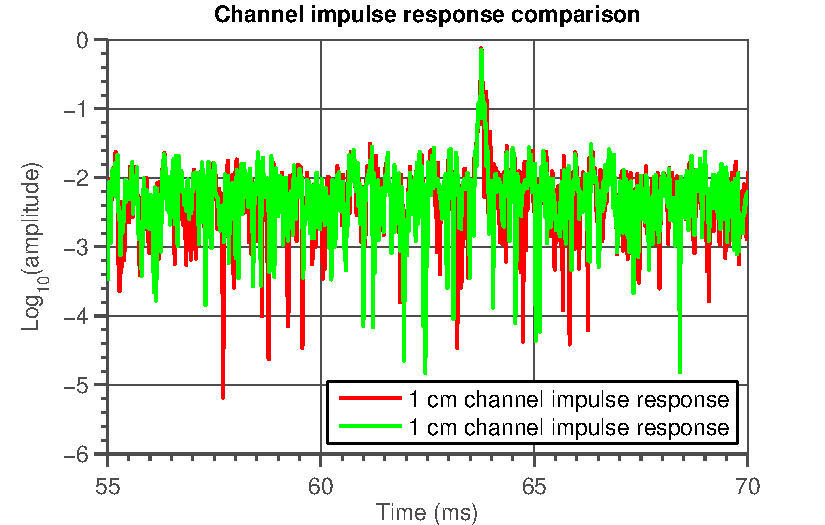
\includegraphics[width=\linewidth]{\figpath/ass-2/report-2-3/ass-2-report-2-impulse-responses-1.pdf}
		\caption{\centering Recovered channel impulse responses through two microphones at the same distance}
	\end{subfigure}
	\begin{subfigure}{.49\textwidth}
		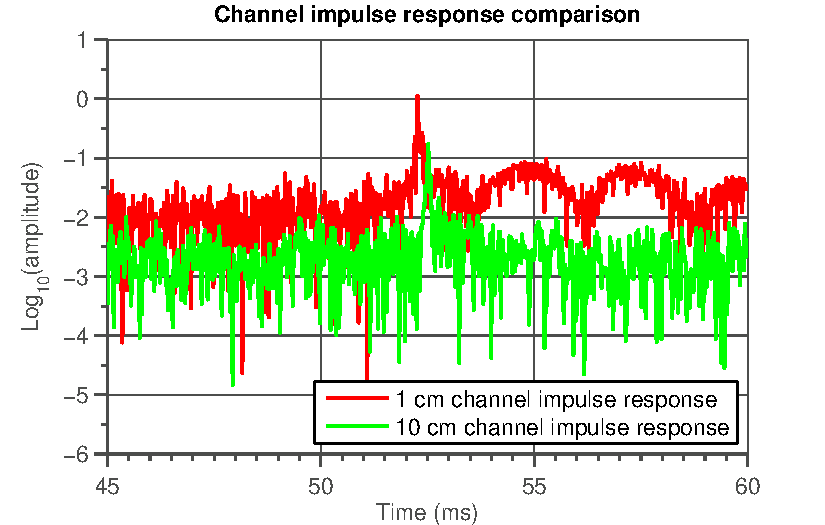
\includegraphics[width=\linewidth]{\figpath/ass-2/report-2-3/ass-2-report-2-impulse-responses-2.pdf}
		\caption{\centering Recovered channel impulse responses through two microphones spaced \SI{9}{cm}}
	\end{subfigure}
	\begin{subfigure}{.49\textwidth}
		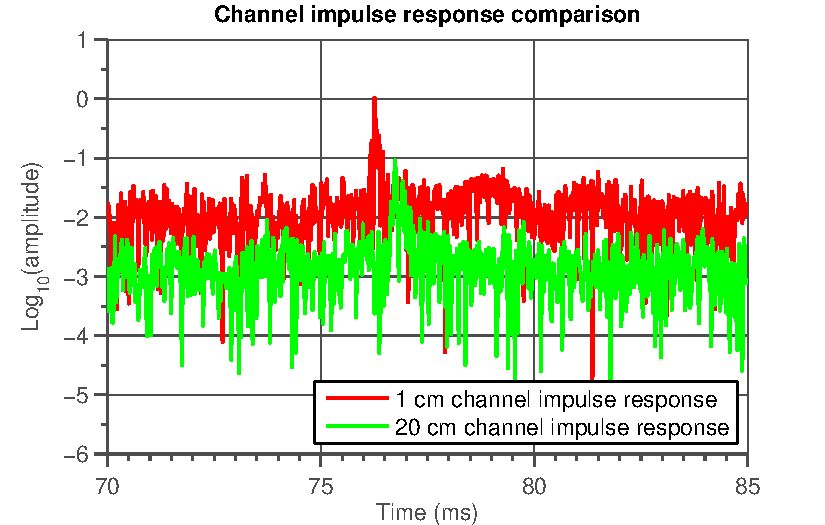
\includegraphics[width=\linewidth]{\figpath/ass-2/report-2-3/ass-2-report-2-impulse-responses-3.pdf}
		\caption{\centering Recovered channel impulse responses through two microphones spaced \SI{19}{cm}}
	\end{subfigure}
	\begin{subfigure}{.49\textwidth}
		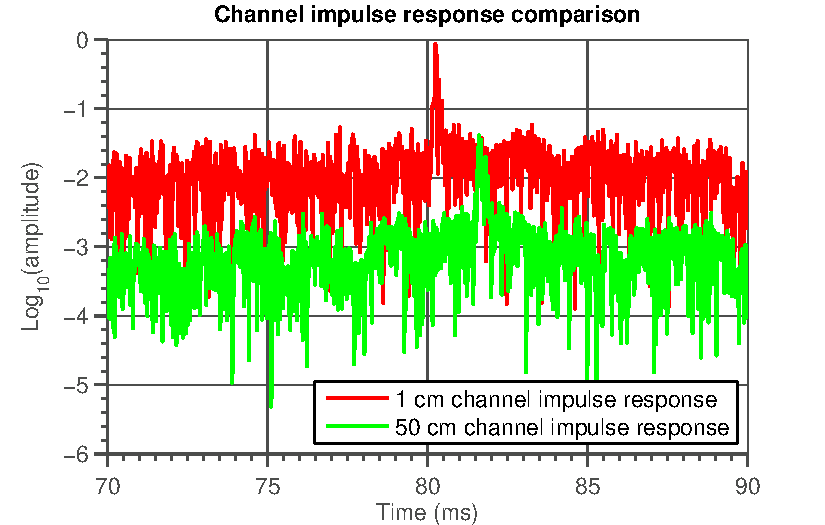
\includegraphics[width=\linewidth]{\figpath/ass-2/report-2-3/ass-2-report-2-impulse-responses-4.pdf}
		\caption{\centering Recovered channel impulse responses through two microphones spaced \SI{49}{cm}}
	\end{subfigure}
	\caption{Recovered channel impulse responses through two microphones spaced various distances}
	\label{fig:ass-2-rep-2-imps}
\end{figure}

The final results are shown in Figure~\ref{fig:ass-2-rep-2-res}. The average error of the determined distances is given by \SI{-7.80}{cm}, and the standard deviation (STD) of the error is given by \SI{2.16}{cm}. The measurements could probabily be improved by a better estimation of the speed of sound.

\begin{figure}[H]
	\centering
	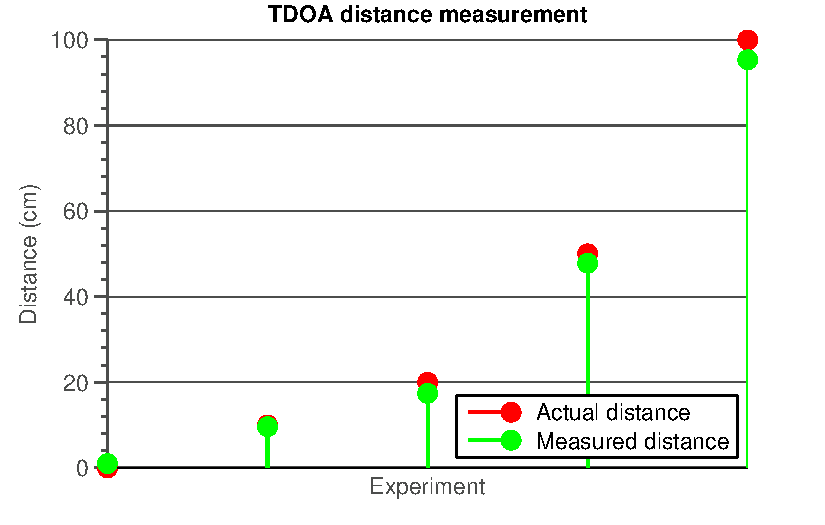
\includegraphics[width=.6\linewidth]{\figpath/ass-2/report-2-3/ass-2-report-2-results.pdf}
	\caption{Determined distances between the microphones}
	\label{fig:ass-2-rep-2-res}
\end{figure}

\subsection{Report 3}
To investigate the stability of the localization algorithm, we recorded several seconds of data to obtain a sequence of microphone spacing estimations. The results are shown in Figure~\ref{fig:ass-2-rep-3}.

\begin{figure}[H]
	\begin{center}
		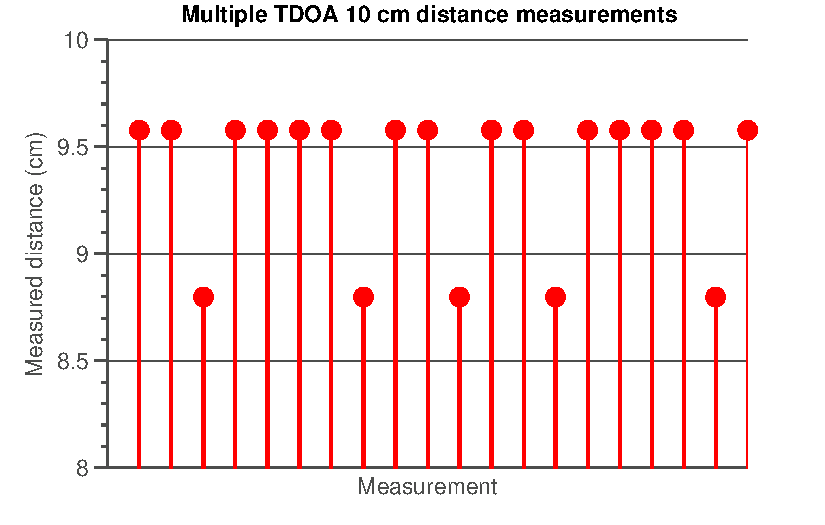
\includegraphics[width=.6\linewidth]{\figpath/ass-2/report-2-3/ass-2-report-3.pdf}
	\end{center}
	\caption{A typical data segment}
	\label{fig:ass-2-rep-3}
\end{figure}

The actual distance between the microphones is \SI{10}{cm}. The mean of estimations of this distance is given by \SI{9.38}{cm} and the STD by \SI{0.35}{cm}. The average error is given by \SI{-0.62}{cm}, which indicates that the estimation is biased. There are no outliers.

We see that all measurements are close to \SI{10}{cm}, but all differ from this value. This is due to fact that the estimation is proportional to the speed of sound. Therefore, uncertainties in the speed of sound directly propagate to the estimated distance. Also, the sampling frequency determines the spatial resolution, which is made obvious by the fact that the measured distances consist of only two different values. The difference between the maximum and minimum measured distance is given by \SI{0.78}{cm}, which perfectly resembles the in Subsection \ref{subsec:ass-2-rep-1} discussed spation resolution.

\subsection{Report 4}
A typical channel impulse response is shown in Figure~\ref{fig:ass-2-rep-4}. Note that the moment of peak detection is indicated by the shown step function.

\begin{figure}[H]
	\begin{center}
		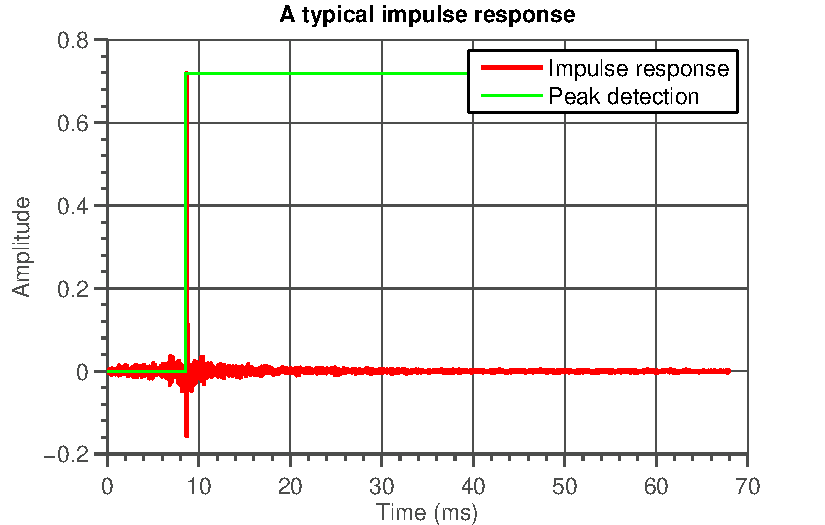
\includegraphics[width=.6\linewidth]{\figpath/ass-2/report-4-5/ass-2-report-4.pdf}
	\end{center}
	\caption{A typical channel impulse response}
	\label{fig:ass-2-rep-4}
\end{figure}

\subsection{Report 5}
Let us consider channel impulse response retrieval through deconvolution by inversion. Let $\mat{X}$ denote the Toeplitz matrix built form the sent signal $x(t)$ and $\vec{y}$ the received signal $y(t)$. Then the channel impulse response esimation $\hat{\vec{h}}$ is given by a least squares solution
\[
	\hat{\vec{h}} = (\tr{\mat{X}} \mat{X})^{-1} \tr{\mat{X}} \vec{y}.
\]
Note that this estimation begins with evaluation of the product $\tr{\mat{X}} \vec{y}$, which can be interpreted as the crosscorrelation $x(-t) \ast y(t)$. If two signals $y_1(t)$ and $y_2(t)$ are received at the same time, then this correlation yields
\[
	x(-t) \ast y(t) = x(-t) \ast y_1(t) + x(-t) \ast y_2(t).
\]
We can conclude that all received signals uncorrelated to the sent signal are removed by the product $\tr{\mat{X}} \vec{y}$. Therefore, received signals uncorrelated to the sent signal do not affect $\hat{\vec{h}}$. This is the reason that all codes ideally need to have a crosscorrelation of zero.
\end{document}